% Provenance (never printed): see sources/outline_sources.md (Year 3:
% speciation and saturation indices; carbonate equilibria applied to rocks;
% weathering kinetics; hydrothermal fluids). Brief: sources/book5/BRIEFS.md,
% ch. 15. Curves from figdata/bachelor-3/carbonate_system.py,
% activity_diagram.py, weathering_rates.py. Exercise and problem values in the
% Book 5 scratch calculator calc/ch15.py. The spring below the Varden
% limestone, its analysis and the granite stream are invented.
\chapter{Interaction eau--roche}\label{ch:b3:water-rock-interaction}

Une source au pied d'un escarpement calcaire laisse une croûte blanche sur chaque
brindille et pierre qu'elle touche~; un ruisseau qui draine un granite transporte de la silice, du sodium
et un peu de potassium, et ne laisse aucune croûte. La différence tient à la
chimie de l'eau, et cette chimie est l'archive de la roche que cette eau a traversée~:
combien de dioxyde de carbone elle transportait, combien de temps elle y est restée, quels
minéraux elle a dissous et ceux qu'elle a construits. Ce chapitre lit cette archive avec
les outils de la chimie des solutions, de l'analyse d'une eau aux vitesses de
dissolution des minéraux et les traces isotopiques des fluides chauds dans la croûte.

\begin{recall}
L'activité, le coefficient d'activité, la force ionique, la spéciation, le produit
de solubilité, l'alcalinité, l'état de saturation $\Omega$, la loi de Henry, les lois de vitesse,
la loi d'Arrhenius, l'état de transition et la valeur $\delta$ figurent dans les
volumes universitaires de chimie. L'altération chimique, l'hydrolyse des
silicates, les minéraux argileux et la kaolinite figurent dans le volume de première année, dans son
chapitre sur l'altération et les argiles~; la lysocline et la profondeur de compensation
des carbonates dans son chapitre sur les sédiments carbonatés, siliceux et évaporitiques. Le
fluide hydrothermal figure dans le volume de deuxième année, dans son chapitre sur les gisements,
et le thermostat de l'altération des silicates dans son chapitre sur le climat au fil
des temps géologiques~; la circulation hydrothermale est dans les manuels scolaires.
\end{recall}

\section{L'analyse d'une eau naturelle}\label{sec:b3:water-rock-interaction:analysis}

Une analyse d'eau énumère les ions majeurs en milligrammes par litre~: calcium,
magnésium, sodium et potassium~; bicarbonate, chlorure, sulfate et nitrate~;
silice dissoute sous forme de \ce{SiO2}~; ainsi que le pH et la température mesurés à la
source, car ces deux valeurs changent dès que l'échantillon la quitte. Diviser par la masse
molaire donne des millimoles par litre, et multiplier par la charge,
milliéquivalents. Une eau diluée est électriquement neutre, si bien que la somme des
cations doit égaler la somme des anions.

\begin{method}[Vérification d'une analyse d'eau]\label{met:b3:water-rock-interaction:analysis}
\begin{enumerate}
\item convertir chaque concentration en \unit{mmol/L} et en \unit{meq/L}~;
\item additionner les cations et les anions en \unit{meq/L}~;
\item calculer l'erreur de bilan de charge $100\,(\sum\text{cat} -
  \sum\text{an})/(\sum\text{cat} + \sum\text{an})$, en pour cent~;
\item accepter l'analyse si l'erreur est inférieure à 1 ou à \qty{2}{\percent} pour une
  eau de 250 à \qty{1000}{mg/L}, un peu plus pour une eau plus diluée~;
  sinon chercher un ion manquant ou une erreur analytique.
\end{enumerate}
\end{method}
% ledger: hem85:charge-balance

L'activité d'un ion est sa molalité multipliée par son coefficient d'activité
$\gamma$. Dans les eaux naturelles, $\gamma$ se calcule à partir de la force ionique $I =
\tfrac12\sum m_i z_i^2$ avec l'équation de Debye--Hückel étendue
\[
-\log\gamma_i = \frac{A z_i^2\sqrt I}{1 + B a_i\sqrt I},
\]
avec $A = 0.5085$ et $B = 0.3281$ pour l'eau à \qty{25}{\celsius}, et une
taille d'ion $a_i$ en ångströms~: 9 pour \ce{H+}, 8 pour \ce{Mg^2+}, 6 pour
\ce{Ca^2+}, 5 pour \ce{CO3^2-}, 4 pour \ce{Na+}, \ce{HCO3-} et \ce{SO4^2-},
3 pour \ce{K+}, \ce{Cl-}, \ce{OH-} et \ce{NO3-}. L'équation reste valable jusqu'à
environ \qty{0.1}{mol/L} de sels monovalents, ce qui couvre les rivières et la plupart des
eaux souterraines, mais non l'eau de mer ni les saumures. La température ne modifie $A$ que de
0.4883 à \qty{0}{\celsius} jusqu'à 0.5425 à \qty{60}{\celsius}, si bien que les valeurs à
\qty{25}{\celsius} conviennent aussi aux eaux froides.
% ledger: hem85:debye-huckel

Le carbone inorganique d'une eau se répartit entre le dioxyde de carbone dissous
(noté \ce{CO2} pour la somme de \ce{CO2} et \ce{H2CO3}), bicarbonate et
carbonate, reliés par
\[
K_1 = \frac{a_{\ce{HCO3-}}\,a_{\ce{H+}}}{a_{\ce{CO2}}}, \qquad
K_2 = \frac{a_{\ce{CO3^2-}}\,a_{\ce{H+}}}{a_{\ce{HCO3-}}}, \qquad
K_H = \frac{a_{\ce{CO2}}}{P_{\ce{CO2}}},
\]
avec $\log K_1 = -6.35$, $\log K_2 = -10.33$ et $\log K_H = -1.47$ à
\qty{25}{\celsius}, et $-6.46$, $-10.49$ et $-1.27$ à \qty{10}{\celsius}
($P$ en atmosphères). Entre pH 6.4 et 10.3, le bicarbonate domine, et dans
la plupart des eaux naturelles, l'alcalinité est presque entièrement due au bicarbonate. Un pH
mesuré et le bicarbonate permettent alors de déduire les deux autres espèces, ainsi que la pression partielle de
dioxyde de carbone avec laquelle l'eau serait en équilibre.
% ledger: phreeqc:carbonate

\section{Saturation}\label{sec:b3:water-rock-interaction:saturation}

\begin{definition}[Indice de saturation]\label{def:b3:water-rock-interaction:si}
L'\emph{indice de saturation}\index{indice de saturation (d'un minéral)}
dans une eau est $\mathrm{SI} = \log(\mathrm{IAP}/K)$, où IAP est
le produit d'activité ionique de l'eau, écrit comme le produit de solubilité
du minéral $K$~: $\mathrm{SI} = \log\Omega$.
\end{definition}

Une eau dont $\mathrm{SI} < 0$ peut dissoudre le minéral, une eau dont
$\mathrm{SI} > 0$ peut le précipiter, et $\mathrm{SI} = 0$ correspond à l'équilibre.
Comme l'énergie libre de la réaction de dissolution vaut $\Delta_r G = RT\ln\Omega
= 2.303\,RT\,\mathrm{SI}$, l'\omterm{def:b3:water-rock-interaction:si}{indice de saturation} mesure aussi la
force motrice, exprimée en unités de $2.303\,RT$, soit environ \qty{5.7}{kJ/mol} à
\qty{25}{\celsius}. Pour la calcite $\mathrm{IAP} = a_{\ce{Ca^2+}}
a_{\ce{CO3^2-}}$ et $\log K = -8.45$ à \qty{25}{\celsius}, $-8.35$ à
\qty{10}{\celsius}~: la calcite est plus soluble dans l'eau froide. Pour le gypse, $\mathrm{SI} = \log(a_{\ce{Ca^2+}}a_{\ce{SO4^2-}}) + 4.55$~;
pour le quartz, dont la dissolution donne \ce{H4SiO4} neutre, $\mathrm{SI} = \log
a_{\ce{H4SiO4}} + 3.98$, et pour la silice amorphe la constante vaut 2.71
au lieu de 3.98. Les indices mesurés portent une incertitude d'au moins $\pm0.1$,
et une eau comprise dans $\pm0.3$ autour de zéro est considérée comme proche de l'équilibre.
% ledger: phreeqc:carbonate, phreeqc:silicates, hem85:si

\section{Équilibres carbonatés dans les roches}\label{sec:b3:water-rock-interaction:carbonate}

La calcite se dissout dans une eau chargée en dioxyde de carbone selon
\[
\ce{CaCO3 + CO2 + H2O <=> Ca^2+ + 2 HCO3-},
\qquad K = \frac{a_{\ce{Ca^2+}}\,a_{\ce{HCO3-}}^2}{P_{\ce{CO2}}}
= \frac{K_{\mathrm{cal}}K_1K_H}{K_2},
\]
avec $\log K = -5.94$ à \qty{25}{\celsius} et $-5.59$ à \qty{10}{\celsius}.
La quantité dissoute dépend de l'origine du dioxyde de carbone.

\begin{definition}[Systèmes carbonatés ouvert et fermé]\label{def:b3:water-rock-interaction:open-closed}
Une eau dissout la calcite dans un \emph{système carbonaté ouvert}\index{système carbonaté ouvert}
lorsqu'elle reste en contact avec un gaz de
$P_{\ce{CO2}}$ fixe, qui remplace le dioxyde de carbone consommé. Elle le fait dans un
\emph{système carbonaté fermé}\index{système carbonaté fermé} lorsqu'elle a d'abord été
chargée en dioxyde de carbone puis isolée du gaz, de sorte que
le dioxyde de carbone qu'elle contient est le seul qu'elle peut utiliser.
\end{definition}

\begin{theorem}[Solubilité de la calcite, systèmes ouvert et fermé]\label{thm:b3:water-rock-interaction:calcite}
Pour une eau de type bicarbonaté calcique, avec $m$ la molalité du calcium,
\[
\text{ouvert~:}\quad m = \left(\frac{K\,P_{\ce{CO2}}}{4\gamma_{\ce{Ca^2+}}
\gamma_{\ce{HCO3-}}^2}\right)^{1/3}~;
\qquad
\text{fermé~:}\quad 4\gamma_{\ce{Ca^2+}}\gamma_{\ce{HCO3-}}^2\,m^3 =
\frac{K_{\mathrm{cal}}K_1}{K_2}\,(C_0 - m),
\]
où $C_0 = K_H P_{\ce{CO2}}$ est le dioxyde de carbone capté avant
la fermeture du système.
\end{theorem}

\begin{proof}
Entre pH 6.5 et 8.5, les ions carbonate, \ce{H+} et \ce{OH-} sont négligeables devant
les ions bicarbonate, donc le bilan de charge s'écrit $2m = m_{\ce{HCO3-}}$. Ouvert~: $K = \gamma
_{\ce{Ca^2+}}m\,\gamma_{\ce{HCO3-}}^2(2m)^2/P_{\ce{CO2}}$, ce qui donne la
racine cubique. Fermé~: chaque calcium dissous consomme un \ce{CO2}, donc $m_{\ce{CO2}}
= C_0 - m$ et $a_{\ce{Ca^2+}}a_{\ce{HCO3-}}^2/a_{\ce{CO2}} = K/K_H =
K_{\mathrm{cal}}K_1/K_2$ donne l'équation du troisième degré.
\end{proof}

Dans le système ouvert, le calcium croît comme la racine cubique de $P_{\ce{CO2}}$~; dans
le système fermé, il est plafonné par $C_0$, et le dioxyde de carbone restant à la
fin, donc la $P_{\ce{CO2}}$ finale, est bien plus faible qu'au départ. L'air du
sol contient de 10 à 100 fois le dioxyde de carbone de l'atmosphère, produit par les
racines et par la décomposition de la matière végétale, et les eaux souterraines présentent couramment
$P_{\ce{CO2}}$ comprise entre $10^{-2.5}$ et $10^{-1}$ atmosphère. L'eau en contact
avec la calcite et l'air ne contient qu'environ \qty{20}{mg/L} de calcium~; la pluie qui
atteint un calcaire en traversant un sol, encore ouvert au gaz du sol, peut en
dissoudre quatre ou cinq fois plus. Le karst est façonné par ce dioxyde de carbone du sol.
% ledger: hem85:pco2, phreeqc:carbonate

Le chemin inverse est le dégazage. Une source qui émerge d'un calcaire transporte
la $P_{\ce{CO2}}$ du sol et de la roche, dix à cent fois celle de
l'air. En système ouvert, elle perd du dioxyde de carbone, le bicarbonate se transforme en
carbonate, le pH monte et l'\omterm{def:b3:water-rock-interaction:si}{indice de saturation} augmente de plus d'une unité,
comme le montre le panneau (b) de la figure ci-dessous, pour la source du
problème du week-end de ce chapitre.
La calcite précipite sur le lit du ruisseau et sur les mousses et les brindilles~: tuf calcaire des
sources froides, travertin des sources chaudes. Les sources qui traversent la roche
rapidement, en quelques jours ou semaines, par des conduits, atteignent couramment la surface
sous-saturées~; celles qui s'infiltrent lentement à travers elle pendant des mois émergent près
de la saturation.
% ledger: hem85:pco2, usgsyvo:travertine

\begin{omfigure}
\begin{tikzpicture}
\begin{groupplot}[group style={group size=2 by 1, horizontal sep=1.6cm},
  omrecord, width=0.47\linewidth, height=0.42\linewidth, title style={font=\small},
  tick label style={font=\scriptsize}, label style={font=\small},
  legend style={font=\scriptsize, legend cell align=left}]
\nextgroupplot[title={(a) solubilité de la calcite},
  xlabel={$\log P_{\ce{CO2}}$ (atm)}, ylabel={calcium dissous (\unit{mmol/L})},
  xmin=-3.5, xmax=-1, ymin=0, ymax=5.5, clip=false,
  xtick={-3.5,-3,-2.5,-2,-1.5,-1}, xticklabels={$-3.5$,$-3$,$-2.5$,$-2$,$-1.5$,$-1$},
  legend style={at={(0.14,0.97)}, anchor=north west}]
\addplot[draw=none, fill=black!6, forget plot] coordinates {(-2.5,0) (-2.5,5.5) (-1,5.5) (-1,0)} -- cycle;
% computed in figdata/bachelor-3/carbonate_system.py
\addplot[omDef, thick] table[x=logp, y=ca_open10] {figdata/out/bachelor-3-carbonate_system-solubility.dat};
\addlegendentry{ouvert, \qty{10}{\celsius}}
\addplot[red!70!black, thick] table[x=logp, y=ca_open25] {figdata/out/bachelor-3-carbonate_system-solubility.dat};
\addlegendentry{ouvert, \qty{25}{\celsius}}
\addplot[omDef, thick, densely dashed] table[x=logp, y=ca_closed10] {figdata/out/bachelor-3-carbonate_system-solubility.dat};
\addlegendentry{fermé, \qty{10}{\celsius}}
\addplot[red!70!black, thick, densely dashed] table[x=logp, y=ca_closed25] {figdata/out/bachelor-3-carbonate_system-solubility.dat};
\addlegendentry{fermé, \qty{25}{\celsius}}
\draw[black, densely dotted] (axis cs:-3.37,0) -- (axis cs:-3.37,5.5);
\node[font=\scriptsize, anchor=south] at (axis cs:-3.37,5.5) {air};
\node[font=\scriptsize, anchor=north] at (axis cs:-1.4,5.45) {eaux souterraines};
\nextgroupplot[title={(b) dégazage de la source},
  xlabel={$\log P_{\ce{CO2}}$ (atm)}, ylabel={indice de saturation de la calcite},
  xmin=-3.5, xmax=-1.5, ymin=-0.2, ymax=1.9, x dir=reverse, clip=false,
  xtick={-3.5,-3,-2.5,-2,-1.5}, xticklabels={$-3.5$,$-3$,$-2.5$,$-2$,$-1.5$}]
% computed in figdata/bachelor-3/carbonate_system.py
\addplot[omDef, thick] table[x=logp, y=si] {figdata/out/bachelor-3-carbonate_system-degassing.dat};
\addplot[black, densely dotted, domain=-3.5:-1.5, samples=2] {0};
\addplot[red!70!black, only marks, mark=*, mark size=1.6pt] table[x=logp, y=si] {figdata/out/bachelor-3-carbonate_system-ends.dat};
\node[font=\scriptsize, anchor=north west] at (axis cs:-1.84,-0.01) {sortie};
\node[font=\scriptsize, anchor=north west] at (axis cs:-3.3,1.55) {air};
\end{groupplot}
\end{tikzpicture}

\par\smallskip{\small (a) Calcium dissous par une eau en équilibre avec
la calcite, en fonction de la pression partielle de dioxyde de carbone (pour le
système fermé, la pression à laquelle l'eau avait été chargée)~: système ouvert en trait plein, système
fermé en pointillés~; l'eau froide dissout davantage~; la bande grise couvre la
gamme des eaux souterraines. (b) La source située sous le calcaire de Varden, à \qty{10}{\celsius},
perdant du dioxyde de carbone en descendant la pente (à lire de gauche à droite, sur un axe inversé)
avant toute formation de calcite~: son calcium et son alcalinité sont fixés, son pH passe
de 7.2 à 8.8, et son \omterm{def:b3:water-rock-interaction:si}{indice de saturation} de 0.04 à 1.6. Constantes d'équilibre
issues d'une base de données publique, coefficients d'activité de Debye--Hückel
étendue.}\label{fig:b3:water-rock-interaction:calcite}
\end{omfigure}
% ledger: phreeqc:carbonate, hem85:debye-huckel, hem85:pco2, data:co2-mlo

Les mêmes réactions chimiques, à l'échelle de l'océan, sont traitées dans les volumes de chimie
de niveau universitaire~: la profondeur à laquelle l'eau de mer devient sous-saturée
en calcite, la lysocline, et la profondeur au-dessous de laquelle la calcite ne
s'accumule plus, sont présentées dans le volume de première année.

\begin{inthefield}[Une source qui construit ses propres terrasses]
\begin{minipage}[t]{0.52\linewidth}\vspace{0pt}
À Palette Spring, l'une des sources de Mammoth Hot Springs, sur le plateau de Yellowstone,
l'eau thermale remonte à travers un calcaire enfoui et le transporte à l'état dissous.
En surface, l'eau s'étale sur ses propres dépôts
et perd du dioxyde de carbone, et le carbonate de calcium précipite sous forme de travertin,
d'abord sur le rebord de chaque bassin, là où l'eau est la plus mince. Les géologues qui étudient
ces sources mesurent un dépôt d'environ trois millimètres par jour, quinze fois la vitesse des tufs
des sources froides. Les bandes orange et brunes
sont des tapis de microbes thermophiles
qui vivent dans les eaux chaudes de ruissellement.
\end{minipage}\hfill
\begin{minipage}[t]{0.44\linewidth}\vspace{0pt}
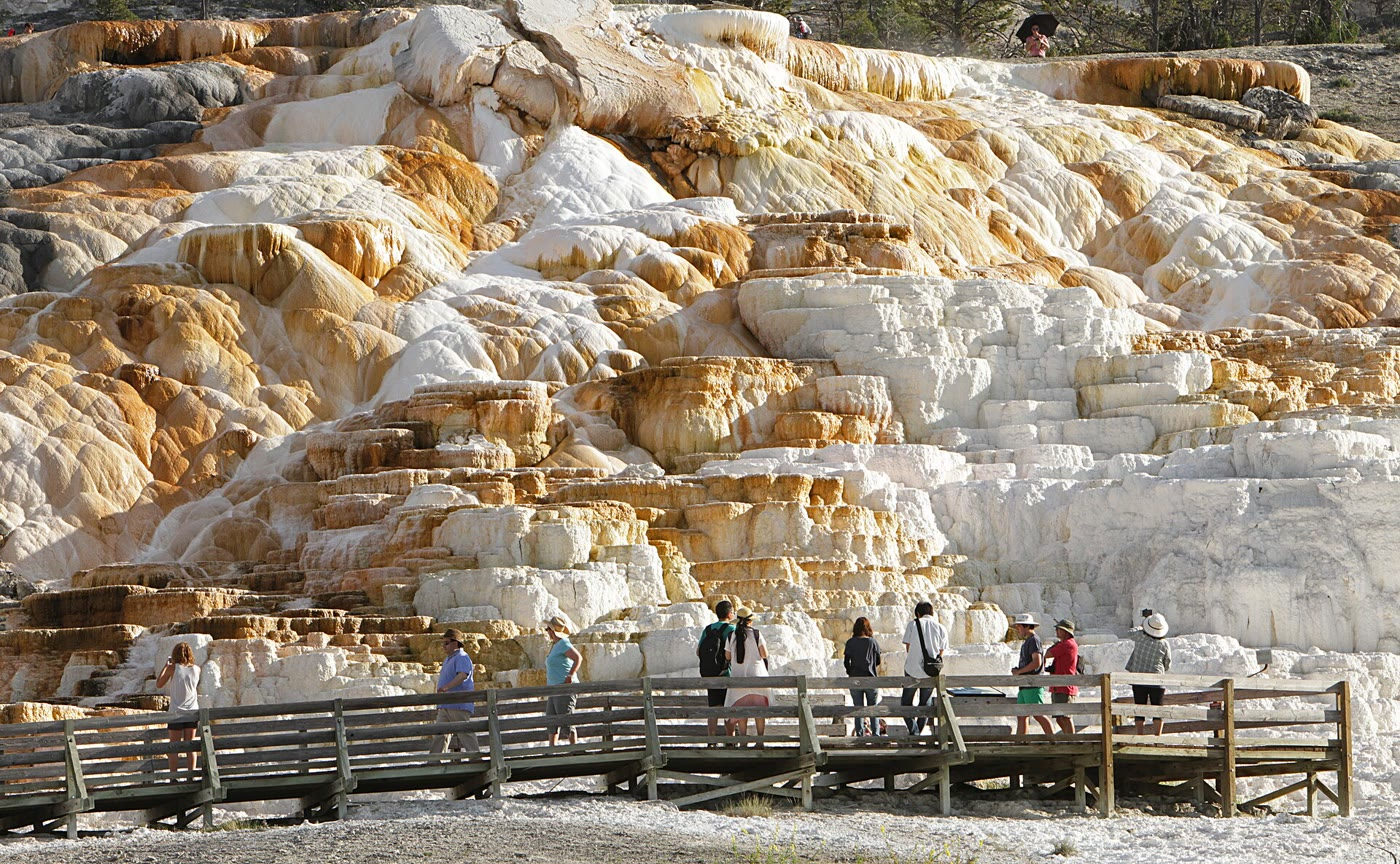
\includegraphics[width=\linewidth]{images/book5/b3-palette-spring-travertine.jpg}

{\scriptsize Terrasses de travertin de Palette Spring, Mammoth Hot Springs, avec
une passerelle et des visiteurs pour l'échelle. Photo NPS de Jim Peaco, domaine public.}
\end{minipage}
\end{inthefield}
% ledger: photo:b3-palette-spring, usgsyvo:travertine, nps:travertine-terraces

\section{Cinétique de l'altération des silicates}\label{sec:b3:water-rock-interaction:kinetics}

Les silicates se dissolvent beaucoup plus lentement que la calcite, et une eau atteint rarement
l'équilibre avec eux~: leur dissolution doit être décrite par une vitesse.

\begin{definition}[Loi de vitesse de dissolution d'un minéral]\label{def:b3:water-rock-interaction:rate-law}
La \emph{loi de vitesse de dissolution d'un minéral}\index{loi de vitesse de dissolution d'un minéral}
donne la vitesse de dissolution par unité de surface minérale, en
\unit{mol.m^{-2}.s^{-1}}, sous la forme d'une somme sur les mécanismes acide, neutre et basique,
\[
r = \sum_j k_j\,e^{-\frac{E_j}{R}\left(\frac1T - \frac1{298.15}\right)}\,
a_{\ce{H+}}^{n_j}\,\bigl(1 - \Omega^{p_j}\bigr)^{q_j},
\]
avec des constantes de vitesse $k_j$ à \qty{25}{\celsius}, des énergies d'activation $E_j$,
des ordres de réaction $n_j$ (négatifs pour le mécanisme basique) et deux exposants
$p_j$, $q_j$, pris en général égaux à 1.
\end{definition}
% ledger: pk04:rate-law

\begin{proposition}[Loin et près de l'équilibre]\label{prop:b3:water-rock-interaction:affinity}
Avec $p = q = 1$, la vitesse ne dépend pas de la saturation de l'eau
lorsque $\Omega \ll 1$, et près de l'équilibre elle est proportionnelle à
l'\omterm{def:b3:water-rock-interaction:si}{indice de saturation}~: $r \approx -2.303\,r_\infty\,\mathrm{SI}$, où
$r_\infty$ est la vitesse loin de l'équilibre.
\end{proposition}

\begin{proof}
Le facteur vaut $1 - \Omega = 1 - 10^{\mathrm{SI}}$. Pour $\mathrm{SI} \ll 0$, il
tend vers 1~; pour $\mathrm{SI}$ voisin de 0, $10^{\mathrm{SI}} \approx 1 +
2.303\,\mathrm{SI}$.
\end{proof}

Les constantes de vitesse proviennent d'expériences de laboratoire sur des poudres minérales fraîches,
réalisées dans des réacteurs à écoulement maintenus loin de l'équilibre. La figure ci-dessous trace
la loi de vitesse pour quatre minéraux à \qty{25}{\celsius}. Chaque courbe a la forme d'un V ou d'un U~:
les protons accélèrent la dissolution dans les eaux acides, les ions hydroxyde dans les eaux basiques, et
entre les deux le mécanisme neutre fixe un plancher. L'olivine se dissout environ trois ordres de grandeur
plus vite que l'albite à pH~5, ce qui explique qu'elle soit le premier des silicates courants à disparaître
d'un sol. Les énergies d'activation de l'albite et de la forstérite, de 65 à
\qty{79}{kJ/mol}, font que leurs vitesses sont quatre à cinq
fois plus rapides à \qty{25}{\celsius} qu'à \qty{10}{\celsius}.
% ledger: pk04:rates

Les vitesses de terrain sont inférieures, de plusieurs ordres de grandeur. Dans des expériences en colonne sur un
granite fraîchement broyé, la vitesse du plagioclase a diminué régulièrement pendant six ans
jusqu'à \qty{7.0e-14}{mol.m^{-2}.s^{-1}}~; le même granite, naturellement altéré et en partie
transformé en kaolinite, s'est dissous à \qty{2.1e-15}{mol.m^{-2}.s^{-1}}
dans les mêmes conditions, et ces deux valeurs restent très supérieures à la vitesse
mesurée dans le profil d'altération lui-même. Sur un grand nombre de minéraux et d'âges, la
vitesse diminue avec le temps $t$ pendant lequel le minéral s'altère, selon $R =
\num{3.1e-13}\,t^{-0.61}$ (mol\,m$^{-2}$\,s$^{-1}$, $t$ en années). Une partie
du ralentissement tient au minéral, dont les surfaces les plus réactives se dissolvent en premier~; le reste
tient au contexte~: eau lente, beaucoup de minéral pour peu de fluide, et eaux
interstitielles proches de l'équilibre, où la proposition ci-dessus rend la
vitesse faible.
% ledger: whitebrantley03:rates

\begin{omfigure}
\begin{tikzpicture}
\begin{axis}[omrecord, width=0.74\linewidth, height=0.46\linewidth,
  xlabel={pH}, ylabel={$\log r$ (\unit{mol.m^{-2}.s^{-1}})},
  xmin=0, xmax=14, ymin=-14.5, ymax=-6, clip=false,
  xtick={0,2,4,6,8,10,12,14}, ytick={-14,-12,-10,-8,-6},
  yticklabels={$-14$,$-12$,$-10$,$-8$,$-6$},
  tick label style={font=\scriptsize}, label style={font=\small},
  legend style={font=\scriptsize, legend cell align=left, at={(1.03,0.5)}, anchor=west}]
% computed in figdata/bachelor-3/weathering_rates.py
\addplot[green!45!black, thick] table[x=ph, y=forsterite] {figdata/out/bachelor-3-weathering_rates-curves.dat};
\addlegendentry{forstérite}
\addplot[omDef, thick] table[x=ph, y=albite] {figdata/out/bachelor-3-weathering_rates-curves.dat};
\addlegendentry{albite}
\addplot[red!70!black, thick, densely dashed] table[x=ph, y=kfeldspar] {figdata/out/bachelor-3-weathering_rates-curves.dat};
\addlegendentry{feldspath K}
\addplot[black, thick, densely dotted] table[x=ph, y=kaolinite] {figdata/out/bachelor-3-weathering_rates-curves.dat};
\addlegendentry{kaolinite}
\end{axis}
\end{tikzpicture}

\par\smallskip{\small Vitesses de dissolution loin de l'équilibre à
\qty{25}{\celsius}, en fonction du pH, d'après une compilation publiée de
paramètres de vitesse de laboratoire. Le pôle olivine, la forstérite, n'a pas de mécanisme basique dans
la compilation~; sa courbe cesse de descendre au plancher neutre.}\label{fig:b3:water-rock-interaction:rates}
\end{omfigure}
% ledger: pk04:rates

\begin{definition}[Régimes d'altération]\label{def:b3:water-rock-interaction:regimes}
L'altération chimique d'un paysage est en \emph{régime limité par
l'apport}\index{régime limité par l'apport} lorsqu'elle est limitée par la vitesse à laquelle
l'érosion apporte des minéraux frais au front d'altération, et dans un
\emph{régime limité par l'altération}\index{régime limité par l'altération} lorsque les
minéraux frais sont abondants et que la vitesse des réactions la limite.
\end{definition}

Une compilation de petits bassins versants montre les deux. Là où l'érosion est lente, sous
des sols épais et lessivés sur un relief doux, le flux d'altération suit le
taux d'érosion~: toute roche fraîche qui arrive est entièrement lessivée, et un climat plus chaud ou
plus humide change peu. Là où l'érosion est rapide, dans les montagnes escarpées, le
flux croît avec le ruissellement, comme la racine carrée du taux d'érosion, et avec
la température, avec une énergie d'activation apparente de $74 \pm
\qty{29}{kJ/mol}$. Seul dans le second régime, l'altération des silicates peut agir comme
thermostat climatique du volume de deuxième année.
% ledger: west05:regimes

Le minéral secondaire qu'une eau d'altération forme se lit sur un autre
diagramme.

\begin{definition}[Diagramme d'activité]\label{def:b3:water-rock-interaction:activity-diagram}
Un \emph{diagramme d'activité}\index{diagramme d'activité (stabilité des minéraux)}
découpe un plan des rapports d'activité d'une eau, tels que
$\log(a_{\ce{K+}}/a_{\ce{H+}})$ en fonction de $\log a_{\ce{H4SiO4}}$, en
domaines où chaque minéral d'un système chimique est stable.
\end{definition}

\begin{proposition}[Frontières d'un diagramme d'activité]\label{prop:b3:water-rock-interaction:boundaries}
Dans le système \ce{K2O}--\ce{Al2O3}--\ce{SiO2}--\ce{H2O}, l'aluminium étant conservé dans les solides
et l'eau à activité unitaire, un minéral comportant $k$ atomes de potassium, $a$ d'aluminium et
$s$ de silicium par formule et de constante de dissolution $K$ (vers \ce{K+},
\ce{Al^3+}, \ce{H4SiO4}) fixe
\[
\log\frac{a_{\ce{Al^3+}}}{a_{\ce{H+}}^3} = \frac{\log K - kX - sY}{a},
\qquad X = \log\frac{a_{\ce{K+}}}{a_{\ce{H+}}},\quad Y = \log a_{\ce{H4SiO4}}.
\]
Le minéral stable donne la plus faible activité d'aluminium, et la frontière
entre deux minéraux est une droite dans $(Y, X)$.
\end{proposition}

\begin{proof}
La dissolution consomme $h = k + 3a$ protons, par bilan de charge, donc $a\log
a_{\ce{Al^3+}} = \log K + h\log a_{\ce{H+}} - k\log a_{\ce{K+}} - s\log
a_{\ce{H4SiO4}}$~; en divisant par $a$ et en passant $3\log a_{\ce{H+}}$ à gauche
donne l'expression. Une eau en équilibre avec un minéral est
sous-saturée vis-à-vis de tout minéral qui exigerait davantage d'aluminium, et
sursaturée vis-à-vis de ceux qui en exigeraient moins, de sorte que le moins soluble est
stable. En égalant deux de ces expressions, linéaires en $X$ et $Y$, on obtient une droite.
\end{proof}

Avec les constantes à \qty{25}{\celsius}, la gibbsite cède la place à la kaolinite pour
$\log a_{\ce{H4SiO4}} = -4.39$ (\qty{2.4}{mg/L} de silice), et la kaolinite cède la
place à la muscovite pour $\log(a_{\ce{K+}}/a_{\ce{H+}}) = 1.55$, et le feldspath potassique
n'est stable que dans les eaux riches en potassium et en silice. Le diagramme est la
séquence d'altération du volume de première année en chiffres~: une eau diluée qui
emporte le potassium et la silice, ramène un feldspath à la gibbsite~; une eau qui
garde davantage de silice forme de la kaolinite~; une eau qui garde davantage de potassium, comme en profondeur,
donne un mica.
% ledger: phreeqc:silicates

\begin{omfigure}
\begin{tikzpicture}
\begin{axis}[omrecord, width=0.66\linewidth, height=0.5\linewidth,
  xlabel={$\log a_{\ce{H4SiO4}}$}, ylabel={$\log(a_{\ce{K+}}/a_{\ce{H+}})$},
  xmin=-6, xmax=-2, ymin=0, ymax=10, clip=false,
  xtick={-6,-5,-4,-3,-2}, xticklabels={$-6$,$-5$,$-4$,$-3$,$-2$},
  tick label style={font=\scriptsize}, label style={font=\small}]
% computed in figdata/bachelor-3/activity_diagram.py
\addplot[black, thick, unbounded coords=jump] table[x=y, y=x] {figdata/out/bachelor-3-activity_diagram-lines.dat};
\addplot[omDef, densely dashed] table[x=y, y=x] {figdata/out/bachelor-3-activity_diagram-quartz.dat};
\addplot[omDef, densely dotted] table[x=y, y=x] {figdata/out/bachelor-3-activity_diagram-amorph.dat};
\addplot[red!70!black, only marks, mark=*, mark size=1.8pt] table[x=y, y=x] {figdata/out/bachelor-3-activity_diagram-samples.dat};
\node[font=\small] at (axis cs:-5.4,0.8) {gibbsite};
\node[font=\small] at (axis cs:-3.25,0.75) {kaolinite};
\node[font=\small] at (axis cs:-4.6,5.0) {muscovite};
\node[font=\small] at (axis cs:-3.3,9.3) {feldspath potassique};
\node[font=\scriptsize, omDef, anchor=south] at (axis cs:-3.98,10) {quartz};
\node[font=\scriptsize, omDef, anchor=south] at (axis cs:-2.71,10) {silice amorphe};
\node[font=\scriptsize, red!70!black, anchor=west] at (axis cs:-4.58,0.38) {A};
\node[font=\scriptsize, red!70!black, anchor=west] at (axis cs:-3.80,1.29) {B};
\node[font=\scriptsize, red!70!black, anchor=west] at (axis cs:-3.48,4.08) {C};
\end{axis}
\end{tikzpicture}

\par\smallskip{\small Domaines de stabilité dans le système
\ce{K2O}--\ce{Al2O3}--\ce{SiO2}--\ce{H2O} à \qty{25}{\celsius}, avec la saturation du quartz
(tirets) et de silice amorphe (pointillés). Trois eaux fictives~: A, un cours d'eau
tropical et dilué~; B, un cours d'eau sur granite~; C, une eau souterraine profonde dans
granite}\label{fig:b3:water-rock-interaction:activity}
\end{omfigure}
% ledger: phreeqc:silicates

\section{Fluides hydrothermaux}\label{sec:b3:water-rock-interaction:hydrothermal}

De l'eau chaude circulant dans la croûte, près d'une dorsale ou d'une intrusion,
échange de l'oxygène avec la roche qu'elle traverse. À haute température, le
fractionnement entre roche et eau est faible, et les deux tendent vers
l'équilibre isotopique~: l'eau météorique, légère, rend la roche plus légère, et l'eau
plus lourde. Le déplacement de la roche mesure la quantité d'eau
ayant circulé.

\begin{definition}[Rapport eau--roche]\label{def:b3:water-rock-interaction:water-rock-ratio}
Le \emph{rapport eau--roche}\index{rapport eau--roche} $W/R$ d'un
système hydrothermal est la masse d'eau ayant échangé avec une masse de
roche, divisée par cette masse de roche.
\end{definition}

\begin{proposition}[Rapports eau--roche à partir des isotopes de l'oxygène]\label{prop:b3:water-rock-interaction:wr}
Soit une roche, de $\delta_r^i$ initial, qui échange de l'oxygène avec une eau de
$\delta_w^i$ initial jusqu'à ce qu'elle atteigne $\delta_r^f$, en équilibre avec l'eau
qu'elle a rencontrée en dernier, $\Delta = \delta_r^f - \delta_w^f$, et soient $c_r$ et $c_w$ les
concentrations en oxygène de la roche et de l'eau. Dans un système clos (un seul lot
d'eau) et dans un système ouvert (eau passant une seule fois),
\[
\frac WR\Big|_{\text{fermé}} = \frac{c_r}{c_w}\,
\frac{\delta_r^f - \delta_r^i}{\delta_w^i - \delta_r^f + \Delta},
\qquad
\frac WR\Big|_{\text{ouvert}} = \frac{c_r}{c_w}\,
\ln\!\left(\frac{\delta_r^f - \delta_r^i}{\delta_w^i - \delta_r^f + \Delta} + 1\right).
\]
\end{proposition}

\begin{proof}
Clos~: l'oxygène~18 se conserve, $c_wW\delta_w^i + c_rR\delta_r^i = c_wW
\delta_w^f + c_rR\delta_r^f$, avec $\delta_w^f = \delta_r^f - \Delta$~; on résout
pour $W/R$. Ouvert~: une portion d'eau $\mathrm dW$ entre à $\delta_w^i$ et ressort en
équilibre avec la roche, à $\delta_r - \Delta$, donc $c_rR\,\mathrm d\delta_r
= c_w(\delta_w^i - \delta_r + \Delta)\,\mathrm dW$. En séparant,
$\int_{\delta_r^i}^{\delta_r^f}\mathrm d\delta_r/(\delta_w^i - \delta_r +
\Delta) = (c_w/c_r)\,W/R$, et l'intégrale vaut $-\ln[(\delta_w^i - \delta_r^f
+ \Delta)/(\delta_w^i - \delta_r^i + \Delta)]$, ce qui donne le résultat annoncé.
\end{proof}

Pour l'oxygène, $c_r/c_w$ vaut environ 0.5. Le système ouvert exige toujours moins
d'eau que le système clos pour un même décalage, car chaque portion ressort
aussi lourde que possible. Autour de nombreuses intrusions, le $\delta^{18}\mathrm O$ de la
roche encaissante dessine une cible de faibles valeurs, allant d'environ $+6$ à
moins de 0, centrée là où le plus d'eau a circulé~; les gisements liés au fluide hydrothermal
sont souvent à l'intérieur de la courbe la plus basse, ce qui fait de la carte un
outil d'exploration.
% ledger: white13c9:water-rock

\begin{omfigure}
\begin{tikzpicture}[font=\small, >=Stealth]
\draw[thick, fill=black!6] (0,0) rectangle (4,2.2);
\node at (2,1.55) {roche, masse $R$};
\node at (2,0.95) {$\delta_r^i \to \delta_r^f$};
\node[font=\scriptsize] at (2,0.4) {échange à la température $T$};
\draw[->, thick, omDef] (-2.6,1.1) -- (-0.1,1.1);
\node[omDef, anchor=south, align=center, font=\scriptsize] at (-1.35,1.15) {eau entrante\\ $\delta_w^i$, $\mathrm dW$};
\draw[->, thick, red!70!black] (4.1,1.1) -- (6.6,1.1);
\node[red!70!black, anchor=south, align=center, font=\scriptsize] at (5.35,1.15) {eau sortante\\ $\delta_r - \Delta$};
\node[anchor=north, font=\scriptsize, align=center] at (2,-0.15) {système ouvert~: chaque portion ne passe qu'une fois et ressort en\\ équilibre avec la roche qu'elle a rencontrée en dernier};
\end{tikzpicture}

\par\smallskip{\small Le modèle en boîte d'un système hydrothermal. Dans un système clos
un seul lot d'eau reste au contact de la roche jusqu'à ce que les deux soient en équilibre~;
dans un système ouvert, l'eau circule à travers la roche, et celle-ci se rapproche
un peu vers l'eau à chaque portion.}\label{fig:b3:water-rock-interaction:box}
\end{omfigure}

\begin{definition}[Modèle de chemin réactionnel]\label{def:b3:water-rock-interaction:reaction-path}
Un \emph{modèle de chemin réactionnel}\index{modèle de chemin réactionnel} suit la
composition d'une eau et des minéraux qu'elle forme au fil de la réaction,
en ajoutant de petites quantités d'un réactif (un minéral qui se dissout, un gaz qui s'échappe,
chaleur retirée) et en recalculant la spéciation et les \omterm{def:b3:water-rock-interaction:si}{indices de saturation} à
chaque étape, en faisant précipiter tout minéral qui atteint la saturation.
\end{definition}

Un \omterm{def:b3:water-rock-interaction:reaction-path}{modèle de chemin réactionnel} appliqué à la source du problème du week-end, avec dégazage
pas à pas, fait précipiter la calcite dès que son indice dépasse zéro~; appliqué à
un granite et une eau de pluie, il forme d'abord de la gibbsite, puis de la kaolinite, puis
de la mica à mesure que l'eau se charge en silice et en potassium, en traçant un chemin à travers le
\omterm{def:b3:water-rock-interaction:activity-diagram}{diagramme d'activité}. Les logiciels de spéciation procèdent ainsi avec des bases de données de
constantes d'équilibre telles que celles utilisées dans ce chapitre.
% ledger: phreeqc:silicates

\section{Exercices}

\begin{exercise}[$\star$]\label{exo:b3:water-rock-interaction:1}
Une eau présente (en \unit{mg/L}) \ce{Ca} 48, \ce{Mg} 9.7, \ce{Na} 23, \ce{K} 3.9,
\ce{HCO3} 183, \ce{Cl} 35.5 et \ce{SO4} 48. Calculer son erreur sur le
bilan ionique. L'analyse est-elle acceptable~?
\end{exercise}

\begin{exercise}[$\star$]\label{exo:b3:water-rock-interaction:2}
À une force ionique de 0.0050, calculer les coefficients d'activité de
\ce{Ca^2+}, \ce{HCO3-} et \ce{SO4^2-}.
\end{exercise}

\begin{exercise}[$\star$]\label{exo:b3:water-rock-interaction:3}
Une eau qui draine une marne gypsifère contient \qty{3.0}{mmol/L} de calcium et
\qty{4.0}{mmol/L} de sulfate, à une force ionique de 0.016. Calculer l'\omterm{def:b3:water-rock-interaction:si}{indice de
saturation} du gypse. L'eau peut-elle encore dissoudre du gypse~?
\end{exercise}

\begin{exercise}[$\star$]\label{exo:b3:water-rock-interaction:4}
Une eau souterraine contient \qty{12}{mg/L} de silice, exprimée en \ce{SiO2} et
présente sous forme de \ce{H4SiO4}. Calculer ses \omterm{def:b3:water-rock-interaction:si}{indices de saturation} pour le quartz et pour
la silice amorphe à \qty{25}{\celsius}.
\end{exercise}
% ledger: phreeqc:silicates

\begin{exercise}[$\star\star$]\label{exo:b3:water-rock-interaction:5}
En prenant les coefficients d'activité égaux à 1, calculer le calcium dissous par un
système ouvert à $P_{\ce{CO2}} = 10^{-2}$~atm à \qty{25}{\celsius} et à
\qty{10}{\celsius}, en \unit{mmol/L} et \unit{mg/L}.
\end{exercise}

\begin{exercise}[$\star\star$]\label{exo:b3:water-rock-interaction:6}
Une eau à \qty{25}{\celsius} a un pH de 7.60 et contient \qty{4.0}{mmol/L} de
bicarbonate. Avec des coefficients d'activité égaux à 1, calculer le
dioxyde de carbone dissous et les carbonates, sa $P_{\ce{CO2}}$ et la part de chaque espèce dans
le carbone inorganique dissous.
\end{exercise}

\begin{exercise}[$\star\star$]\label{exo:b3:water-rock-interaction:7}
Un grain d'albite est une sphère de \qty{1}{mm} de diamètre dans une eau du sol de pH 5 à
\qty{25}{\celsius}, qui se dissout à la vitesse de la figure, $\log r = -12.09$.
Avec un volume molaire de \qty{101.31}{cm^3/mol}, à quelle vitesse son rayon
diminue-t-il, et combien de temps dure ce processus~?
\end{exercise}
% ledger: pk04:rates, phreeqc:silicates

\begin{exercise}[$\star\star$]\label{exo:b3:water-rock-interaction:8}
Par quel facteur la vitesse de dissolution neutre de l'albite ($E =
\qty{69.8}{kJ/mol}$) croît-elle de \qty{5}{\celsius} à \qty{25}{\celsius}~? Et par
quel facteur un flux d'altération avec $E = \qty{74}{kJ/mol}$~?
\end{exercise}
% ledger: pk04:rates, west05:regimes

\begin{exercise}[$\star\star$]\label{exo:b3:water-rock-interaction:9}
Établir la frontière kaolinite--muscovite du \omterm{def:b3:water-rock-interaction:activity-diagram}{diagramme d'activité} à partir des
constantes $\log K = 7.435$ (kaolinite, 2 Al, 2 Si) et $12.703$ (muscovite, 1
K, 3 Al, 3 Si). Une eau à \qty{25}{\celsius} contient \qty{2.0}{mg/L} de
potassium, \qty{15}{mg/L} de silice et un pH de 7.0~: quel minéral se forme-t-il~?
\end{exercise}
% ledger: phreeqc:silicates

\begin{exercise}[$\star\star\star$]\label{exo:b3:water-rock-interaction:10}
Près d'une intrusion, une granodiorite de $\delta^{18}\mathrm O = +6$ est
relevée à $-2$ (\unit{\permil}). L'eau météorique présentait $-13$, et à la
température d'échange, la roche était \qty{2}{\permil} plus lourde que
l'eau. Avec $c_r/c_w = 0.5$, calculer le \omterm{def:b3:water-rock-interaction:water-rock-ratio}{rapport eau--roche} pour un système
clos et pour un système ouvert, et expliquer pourquoi ils diffèrent.
\end{exercise}
% ledger: white13c9:water-rock

\begin{exercise}[$\star\star\star$]\label{exo:b3:water-rock-interaction:11}
De la pluie chargée de gaz du sol, à $P_{\ce{CO2}} = 10^{-1.5}$~atm et
\qty{10}{\celsius}, atteint un calcaire. Avec des coefficients d'activité de 1,
calculer le calcium qu'elle dissout si elle reste ouverte au gaz du sol et si elle
est d'abord isolée de ce gaz. Quelle fraction de son dioxyde de carbone
reste dans le cas fermé, et quelle est sa $P_{\ce{CO2}}$ finale~?
\end{exercise}

\begin{exercise}[$\star\star\star$]\label{exo:b3:water-rock-interaction:12}
En utilisant la proposition sur les vitesses près de l'équilibre, quelle fraction
de la vitesse loin de l'équilibre à laquelle un minéral se dissout pour $\mathrm{SI} =
-2$, $-1$ et $-0.1$~? Une vitesse de laboratoire mesurée après 6 ans de réaction
suit la loi puissance du chapitre~: de quel facteur elle aura diminué
après \num{10000} ans~? Combiner les deux effets pour expliquer pourquoi les vitesses de terrain sont
si faibles.
\end{exercise}
% ledger: whitebrantley03:rates

\section{Problème~: la source sous le calcaire de Varden}

\begin{problem}[{Problème du week-end --- l'analyse, le dioxyde de carbone et
la saturation d'une source fictive issue d'un calcaire, et d'un ruisseau granitique}]
\label{pb:b3:water-rock-interaction:1}
Une source jaillit au pied du calcaire jurassique des collines de Varden, à
\qty{10}{\celsius} et de pH 7.20. Son analyse donne (en \unit{mg/L})~: \ce{Ca}
112, \ce{Mg} 4.0, \ce{Na} 7.0, \ce{K} 1.2, \ce{HCO3} 340, \ce{Cl} 11,
\ce{SO4} 14, \ce{NO3} 9. À \qty{10}{\celsius}~: $\log K_{\mathrm{cal}} =
-8.35$, $\log K_1 = -6.46$, $\log K_2 = -10.49$, $\log K_H = -1.27$. Utiliser
l'équation de Debye--Hückel étendue du chapitre, négliger les paires d'ions et prendre
pour l'air $\log P_{\ce{CO2}} = -3.37$.

\medskip\noindent\textbf{Partie I --- L'analyse.}
\begin{enumerate}
\item Convertir l'analyse en \unit{mmol/L}.
\item Calculer l'erreur de bilan de charge. L'analyse est-elle acceptable~?
\item Calculer la force ionique.
\item Calculer les coefficients d'activité de \ce{Ca^2+}, \ce{HCO3-} et
  \ce{CO3^2-}.
\item L'équation de Debye--Hückel étendue est-elle valide ici~?
\end{enumerate}

\medskip\noindent\textbf{Partie II --- Dioxyde de carbone.}
\begin{enumerate}[resume]
\item Calculer l'activité de l'hydrogénocarbonate.
\item Calculer l'activité du dioxyde de carbone dissous.
\item Calculer la $P_{\ce{CO2}}$ de la source. Combien de fois est-elle supérieure
  à celle de l'air, et d'où peut venir le dioxyde de carbone~?
\item Calculer la concentration en carbonates et la part de chaque espèce dans
  le carbone inorganique dissous.
\item Vérifier que l'alcalinité est presque entièrement due à l'hydrogénocarbonate.
\end{enumerate}

\medskip\noindent\textbf{Partie III --- Saturation et travertin.}
\begin{enumerate}[resume]
\item Calculer le produit d'activité ionique et l'\omterm{def:b3:water-rock-interaction:si}{indice de saturation} de la calcite
  à l'exutoire.
\item La source est-elle à l'équilibre avec la calcite~? S'agit-il d'une source de conduit ou
  d'une résurgence lente et diffuse~?
\item Calculer le calcium d'un système ouvert à l'équilibre avec la calcite à
  la $P_{\ce{CO2}}$ de la source, avec les coefficients d'activité de la question~4,
  et comparer avec l'analyse.
\item L'eau dégaze dans l'air avant toute formation de calcite. En gardant la
  activité de l'hydrogénocarbonate inchangée, calculer son pH et son \omterm{def:b3:water-rock-interaction:si}{indice de saturation}.
\item Estimer le calcium conservé une fois que la calcite a reprécipité pour
  retrouver l'équilibre avec l'air (système ouvert, coefficients d'activité à la nouvelle
  force ionique $3m$), et la masse de calcite par litre.
\item La source débite \qty{2.0}{L/s} et étale son dépôt sur
  \qty{400}{m^2}. Si toute cette calcite restait en place, avec une masse volumique de
  \qty{2.71}{g/cm^3}, à quelle vitesse croîtrait le dépôt~?
\end{enumerate}

\medskip\noindent\textbf{Partie IV --- Le ruisseau granitique.} Un ruisseau sur le
granite de Varden, sous un sol épais sur des pentes douces, présente (à
\qty{25}{\celsius}) \qty{1.2}{mg/L} de potassium, \qty{9.0}{mg/L} de
silice et un pH de 5.8.
\begin{enumerate}[resume]
\item Calculer sa position sur le \omterm{def:b3:water-rock-interaction:activity-diagram}{diagramme d'activité}.
\item Quel minéral se forme-t-il~? Calculer son \omterm{def:b3:water-rock-interaction:si}{indice de saturation} pour le quartz.
\item En dessous de quelle concentration en silice l'eau formerait-elle de la gibbsite~?
\item À quel pH atteindrait-elle la frontière kaolinite--muscovite~?
\item Calculer la vitesse de dissolution du feldspath potassique dans cette eau, loin de
  l'équilibre, à partir des paramètres $\log k = -10.06$, $n = 0.500$ (acide)~;
  $-12.41$ (neutre)~; $-21.20$, $n = -0.823$ (basique).
\item L'altération de ce bassin versant relève-t-elle plutôt d'un \omterm{def:b3:water-rock-interaction:regimes}{régime limité par l'apport} ou
  limité par l'altération~? Pourquoi~?
\item Avec une énergie d'activation apparente de \qty{74}{kJ/mol}, de quel facteur
  varierait un flux limité par l'altération entre \qty{10}{\celsius} et
  \qty{25}{\celsius}~?
\item Donner l'\omterm{def:b3:water-rock-interaction:si}{indice de saturation} de la calcite de l'eau de la source à son
  exutoire.
\end{enumerate}
\end{problem}
% ledger: phreeqc:carbonate, phreeqc:silicates, hem85:debye-huckel, hem85:charge-balance, hem85:si, hem85:pco2, pk04:rates, west05:regimes, data:co2-mlo
